\documentclass[english,14pt]{beamer}
\usetheme{EastLansing}
\usecolortheme{spruce}

\usepackage{xcolor}
\usepackage{listings}
\usepackage{courier}
\usepackage{graphicx}
\usepackage{amsmath}
\usepackage{algorithm2e}
\usepackage{multicol}
\usepackage{hyperref}

% http://mirrors.ibiblio.org/CTAN/macros/latex/contrib/datetime2/datetime2.pdf
\usepackage{babel}
\usepackage[useregional]{datetime2}

% https://tex.stackexchange.com/questions/42619/x-mark-to-match-checkmark
\usepackage{pifont}% http://ctan.org/pkg/pifont

%% https://stackoverflow.com/questions/1435837/how-to-remove-footers-of-latex-beamer-templates
%%gets rid of bottom navigation bars
%\setbeamertemplate{footline}[page number]
%
%gets rid of navigation symbols
\setbeamertemplate{navigation symbols}{}


\usefonttheme[onlymath]{serif}

\definecolor{mGreen}{rgb}{0,0.6,0}
\definecolor{mGray}{rgb}{0.5,0.5,0.5}
\definecolor{mPurple}{rgb}{0.8,0,0.82}
\definecolor{backgroundColour}{rgb}{0.95,0.95,0.92}
\definecolor{lightBlue}{rgb}{0.1, 0.1, 0.8}

\newcommand\red[1]{{\color{red} #1}}
\newcommand\green[1]{{\color{green} #1}}
\newcommand\blue[1]{{\color{blue} #1}}

\newcommand{\cmark}{\ding{51}}%
\newcommand{\xmark}{\ding{55}}%

\lstdefinestyle{CStyle}{
    backgroundcolor=\color{backgroundColour},   
    commentstyle=\color{mGreen},
    keywordstyle=\color{magenta},
    numberstyle=\tiny\color{mGray},
    stringstyle=\color{mPurple},
    basicstyle=\footnotesize,
    breakatwhitespace=false,         
    breaklines=true,                 
    captionpos=b,                    
    keepspaces=true,                 
    numbers=left,                    
    numbersep=5pt,                  
    showspaces=false,                
    showstringspaces=false,
    showtabs=false,                  
    tabsize=2,
    language=C
}

\lstdefinestyle{pseudo}{
        basicstyle=\ttfamily\footnotesize,
        keywordstyle=\color{lightBlue},
        morekeywords={BEGIN,END,IF,ELSE,ENDIF,ELSEIF,PRINT,WHILE,RETURN,ENDWHILE,DO,FOR,TO,IN,ENDFOR,BREAK,INPUT},
        morecomment=[l]{//},
        commentstyle=\color{mGreen}
}

\lstset{basicstyle=\footnotesize\ttfamily,breaklines=true}
\lstset{framextopmargin=50pt,tabsize=2}

\title{ENGG1003 - Thursday Week 3}
\subtitle{Review of Monday's lecture \\ \& overview of Week 4 assessed lab}
\author{Steve Weller}
\institute{University of Newcastle}
%\date{\today}
\date{11 March, 2021}

% following is a bit of a hack, but forces page numbers (technically: frame numbers) to run 1,2,3,... 
% with titlepage counting as frame 1

\addtocounter{framenumber}{1}
\titlepage

\begin{document}

\begin{flushleft}
{\scriptsize Last compiled:~\DTMnow}
\vspace*{-5mm}
\end{flushleft}
\framebreak

%==============================================================

\begin{frame}[fragile]

\frametitle{Lecture overview}
\begin{enumerate}
	\item Review of Monday's lecture
		\begin{itemize}
			\item \texttt{if}-\texttt{elif}-\texttt{else} 
			\item \texttt{for} loop
			\item \texttt{while} loop
		\end{itemize}

	\item[]
	
	\item Overview of Week 4 assessed lab
	\begin{itemize}
		\item review of main topics covered in weeks 1--3
		\item what to expect in assessed lab
		\item reminder: worth $5$\% of overall course grade
	\end{itemize}	
						
\end{enumerate}

\end{frame}

%==============================================================

\begin{frame}[fragile]

\frametitle{$1)$ Review of Monday's lecture}

Reminder of main ideas in Monday's lecture:

\begin{itemize}
	\item Branching: \textbf{\texttt{if}}, \textbf{\texttt{elif}} and \textbf{\texttt{else}}
	\begin{itemize}
		\item conditional execution of code blocks
		\begin{itemize}
			\item \texttt{if}
			\item \texttt{if}-\texttt{else}
			\item \texttt{if}-\texttt{elif}-\texttt{else}
		\end{itemize}
	\end{itemize}
	
	\item[]
	
	\item Iteration using \textbf{\texttt{for}} loop
	\begin{itemize}
		\item fixed number of iterations
	\end{itemize}

	\item[]
	
	\item Iteration using \textbf{\texttt{while}}
		\begin{itemize}
			\item keep iterating whenever a Boolean condition is satisfied
		\end{itemize}
		
\end{itemize}

\end{frame}

%==============================================================

\begin{frame}[fragile]

\frametitle{}

\frametitle{Branching: \texttt{if}}

\textbf{Example 1}\\
\vspace*{5mm}
Write a Python program which takes an integer $N \in \{1,2,3,4,5,6\}$ and displays a message as follows:

\begin{itemize}
\item $N=1$, display ``You win a prize!''
\item $N \in \{2,3,4,5,6\}$, no message is displayed
\end{itemize}

\vspace*{5mm}

\begin{itemize}
	\item Live demo
\end{itemize}
	
\end{frame}

%==============================================================

\begin{frame}[fragile]

\frametitle{Python code and output for Example 1}

\begin{figure}[ht]
	\centering
	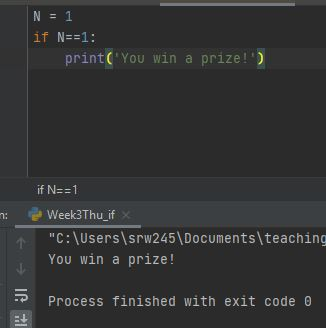
\includegraphics[width=0.6\textwidth]{figures/Week3ThuEx1a}
\end{figure}

\end{frame}

%==============================================================

\begin{frame}[fragile]

\frametitle{Branching: \texttt{if}-\texttt{elif}-\texttt{else}}

\textbf{Example 2}\\
\vspace*{5mm}
Write a Python program which takes an integer $N \in \{1,2,3,4,5,6\}$ and displays a message as follows:

\begin{itemize}
\item $N=1$, display ``You win first prize!''
\item $N=2$, display ``You win second prize!''
\item $N \in \{3,4,5,6\}$, display ``Sorry, no prize''
\end{itemize}

\vspace*{5mm}

\begin{itemize}
	\item Live demo
\end{itemize}
	
\end{frame}

%==============================================================

\begin{frame}[fragile]

\frametitle{Python code and output for Example 2}

\begin{figure}[ht]
	\centering
	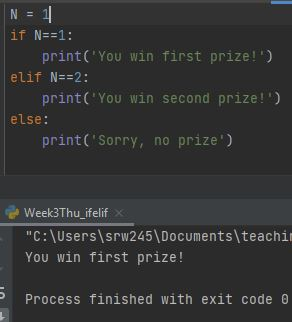
\includegraphics[width=0.5\textwidth]{figures/Week3ThuEx2a}
\end{figure}

\end{frame}

%==============================================================

\begin{frame}[fragile]

\frametitle{}

\frametitle{Iteration using \texttt{for} loop}

\textbf{Example 3}\\
\vspace*{5mm}
Write a Python program which uses a \textbf{\texttt{for}} loop to print the numbers $1, 2, 3, \ldots, 10$ to the console. \\
\vspace*{5mm}

Your program should use the basic form of \texttt{for} loop
\begin{itemize}
	\item ie: in loop header, use \verb+[1,2,3,4,5,6,7,8,9,10]+
\end{itemize}

\vspace*{10mm}

\begin{itemize}
	\item Live demo
\end{itemize}
	
\end{frame}

%==============================================================

\begin{frame}[fragile]

\frametitle{Python code and output for Example 3}

\begin{figure}[ht]
	\centering
	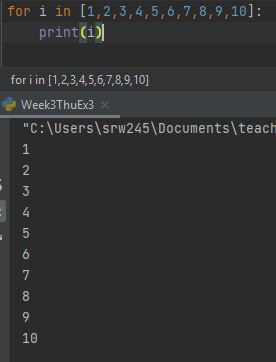
\includegraphics[width=0.4\textwidth]{figures/Week3ThuEx3}
\end{figure}

\end{frame}

%==============================================================

\begin{frame}[fragile]

\frametitle{}

\textbf{Example 4}\\
\vspace*{5mm}
Modify your solution to Example~3 to use a \textbf{\texttt{for}} loop to print the \red{\emph{squares}} of the numbers $1, 2, 3, \ldots, 10$ to the console using the following display format:
\begin{verbatim}
1**2 = 1
2**2 = 4
3**2 = 9
4**2 = 16
.
.
.
10**2 = 100
\end{verbatim}

\begin{itemize}
	\item Live demo
\end{itemize}
	
\end{frame}

%==============================================================

\begin{frame}[fragile]

\frametitle{Python code and output for Example 4}

\begin{figure}[ht]
	\centering
	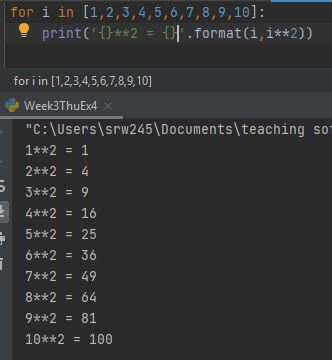
\includegraphics[width=0.5\textwidth]{figures/Week3ThuEx4}
\end{figure}

\end{frame}

%==============================================================

\begin{frame}[fragile]

\frametitle{}

\frametitle{}

\textbf{Example 5}\\
\vspace*{5mm}
Modify your solution to Example~4 to use a \textbf{\texttt{for}} loop to print the squares of the numbers $1, 2, 3, \ldots, \red{1000}$ to the console using the display format in Example 4. You \emph{must} use the \texttt{range} function in the \texttt{for} loop header.
\begin{verbatim}
1**2 = 1
2**2 = 4
3**2 = 9
4**2 = 16
...
1000**2 = 1000000
\end{verbatim}

\begin{itemize}
	\item Live demo
\end{itemize}
	
\end{frame}

%==============================================================

\begin{frame}[fragile]

\frametitle{Python code and output for Example 5}

\begin{figure}[ht]
	\centering
	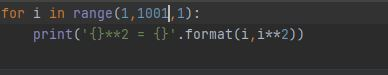
\includegraphics[width=0.5\textwidth]{figures/Week3ThuEx5a}\\
	\vspace*{5mm}
	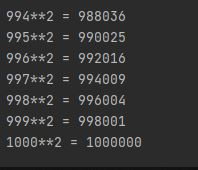
\includegraphics[width=0.5\textwidth]{figures/Week3ThuEx5b}
\end{figure}

\end{frame}

%%==============================================================
%
%\begin{frame}[fragile]
%
%\frametitle{Reflections on Examples 1--5}
%
%\begin{itemize}
%	\item xxx
%	\item[]
%	\item xxx
%\end{itemize}
%\end{frame}

%==============================================================

\begin{frame}[fragile]

\frametitle{Iteration using \texttt{while} loop}

\textbf{Example 6}\\
\vspace*{5mm}
Write a Python program which calculates the sum of the squares of the first $N$ integers:
\[
S_N = 1^2 + 2^2 + 3^2 + \cdots + N^2
\]

\begin{itemize}
	\item your program \emph{must} use a \texttt{while} loop
	\item demonstrate your program for $N=10$
	\item check your answer is correct using the formula
	\[
		S_N = \frac{N(N+1)(2N+1)}{6}
	\]

\end{itemize}

\end{frame}

%==============================================================

\begin{frame}[fragile]

\frametitle{How do we start to solve this problem?}

\begin{itemize}
	\item Don't try and solve the whole problem at once!
	\item[]
	\item Start small and build up your code one small step at a time
	\begin{itemize}
		\item \ldots testing along the way
	\end{itemize}
	\item[]
	\item Suggested first step: display $1,2,3,\ldots,10$ to the console
	\begin{itemize}
		\item tests that your \texttt{while} loop syntax is correct
	\end{itemize}
	\item[]
	\item Coding in small steps often helps in better understanding the problem
\end{itemize}

\end{frame}

%==============================================================

\begin{frame}[fragile]

\frametitle{Python code and output for Example 6}

\begin{figure}[ht]
	\centering
	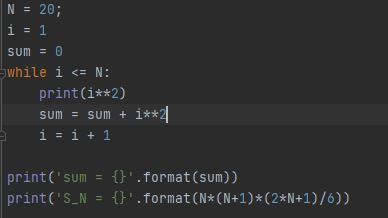
\includegraphics[width=0.5\textwidth]{figures/Week3ThuEx6a}\\
	\vspace*{2mm}
	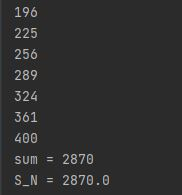
\includegraphics[width=0.3\textwidth]{figures/Week3ThuEx6b}
\end{figure}

\end{frame}

%==============================================================

\begin{frame}[fragile]

\frametitle{$2)$ Overview of assessed lab in week 4}

Key topics we've covered in the course so far:

\vspace*{5mm}

\begin{enumerate}
	\item Python program with library function
	\item Simple plotting
	\item Simple printing
	\item Arrays
	\item Branching: \texttt{if}-\texttt{elif}-\texttt{else}
	\item Looping: \texttt{for} and \texttt{while}
\end{enumerate}

\end{frame}

%==============================================================

\begin{frame}[fragile]

\frametitle{Assessed lab in week 4}

\begin{itemize}
	\item Each student assessed in the face-face lab sessions
	\item Worth $5$\% towards course grade
	\item $5$ marks in lab sheet
	\item Two questions
	\item Answer both questions
	\item Sample paper will shortly be in BB $>$ course materials $>$ week 3 
\end{itemize}

\end{frame}

%==============================================================

\begin{frame}[fragile]

\frametitle{Assessed lab in week 4}

\vspace*{-10mm}
\begin{figure}[ht]
	\centering
	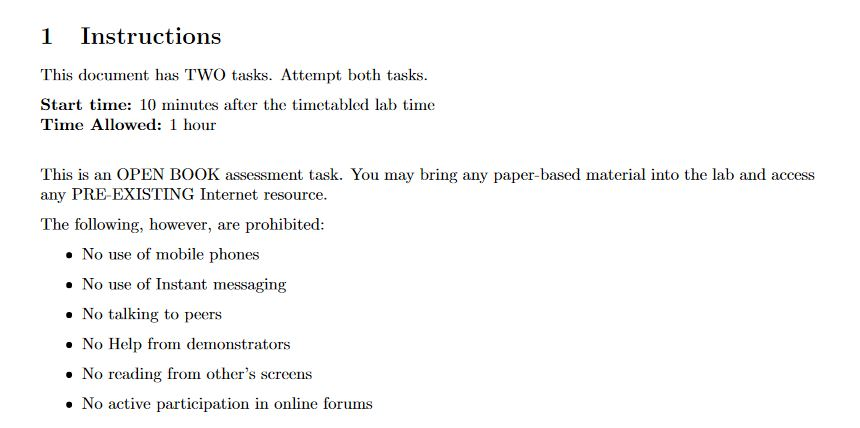
\includegraphics[width=1.05\textwidth]{figures/AssessedLab1Cover}
\end{figure}

\end{frame}

\end{document}